\documentclass{statsmsc}
\usepackage[
  bottom=0.2in,
  left=3cm, right=3cm,
  includefoot
]{geometry}
\title{Model Checking in Bayesian Survival Analysis: A Case Study on Employee Turnover and the Observation Window}
\author{Jing Zhang}
\CID{06014353}
\supervisor{Daniel Mortlock}
%For today's date, use:
\date{\today}
\logoimg{}

% THIS IS WHERE NEW COMMANDS CAN BE DEFINED

% commands below only used in the proof; otherwise can be deleted
\newcommand{\consta}{a}
\newcommand{\X}{X}
\newcommand{\EE}[1]{ \mathrm{E} [ #1 ] }
\newcommand{\inparenth}[1]{\left( #1 \right)}
\usepackage{xcolor}
\usepackage{hyperref}
\hypersetup{
    colorlinks,
    linkcolor={blue!50!black},
    citecolor={blue!50!black},
    urlcolor={blue!50!black}
}
\usepackage{tikz}
\usetikzlibrary{positioning, arrows.meta, shapes.geometric}
\usepackage{enumitem}
\usepackage[most]{tcolorbox}
\tcbuselibrary{listings, breakable}
\usepackage{graphicx}
\usepackage{subcaption}
\usepackage{mathtools} 
\usepackage{booktabs}


\begin{document}

% Generates the Title Page
\maketitle

% Generates plagiarism declaration
\declarationname{Jing Zhang}
\declarationdate{\today}%if you choose to use footnotes, do so sparingly.
\declaration 


\begin{acknowledgements}
I am sincerely indebted to my supervisor, Professor Daniel Mortlock, whose insightful advice and steady support greatly shaped this work. I would also like to acknowledge the encouragement of my fellow MSc Statistics students, as well as the patience and understanding of my family throughout this research journey.
\end{acknowledgements}
\clearpage

\begin{abstract}
This thesis explores model checking in Bayesian survival analysis, using employee turnover data as a motivating case. The dataset records the tenure of 1,129 employees, providing a setting where censoring and observation windows strongly influence inference.

We develop a Bayesian framework that treats the observation window as an estimable parameter, allowing its structural role in censoring to be explicitly evaluated. A key theoretical result emerges: the marginal posterior of the event-rate parameter $\lambda$ is unaffected by prior choices on the observation window $A$, provided $A \geq y_{\max}$. This unusual separability underscores the robustness of inference on $\lambda$ despite model extension.

Posterior predictive model checking, however, reveals that the exponential model with constant hazard fails to capture the “early steep, later flat” turnover pattern, systematically underestimating mid-range events. This mismatch highlights the limits of constant hazards and demonstrates the value of Bayesian model checking not only in diagnosing misfit but also in guiding model improvement.

Overall, the study shows how Bayesian model checking can both advance survival methodology and provide actionable insights into workforce turnover.
\end{abstract}

\setcounter{tocdepth}{2} 
\tableofcontents
\clearpage
%=================================================================

\mainmatter
%==============================================================

%===============================================================
%

\section{Introduction}
The analysis of survival time has a long intellectual history, from the population censuses of the Western Han dynasty in China and the “Yellow Registers” of the Ming dynasty~\cite{von2012household}, to John Graunt’s mortality tables during the London plague in the 17th century~\cite{doi:10.1177/09677720221079826}. These efforts, though rudimentary, already showed how survival data could inform decisions. Modern survival analysis, however, took shape in the mid-20th century with the emergence of parametric, nonparametric, and semiparametric approaches. Parametric models such as the exponential or Weibull~\cite{ibrahim2013bayesian} were among the earliest, assuming specific hazard forms that make inference straightforward but rely on restrictive distributional assumptions. The Kaplan–Meier estimator (1958)~\cite{liu2012survival, kleinbaum1996survival} then introduced a fully nonparametric method for censored data, providing intuitive survival curves without distributional assumptions, though it cannot incorporate covariates. The Cox proportional hazards model (1972)~\cite{Efron01091977, liu2012survival} built on this by combining covariate effects with an unspecified baseline hazard, becoming the standard in biomedical research despite its reliance on the proportional hazards assumption. Together, these models established the classical toolbox that remains central to medicine, epidemiology, and reliability engineering.

Yet this toolbox has limitations. Traditional inference via maximum or partial likelihood~\cite{bartovs2022informed, kalbfleisch2002statistical} provides only point estimates, which can be highly unstable under heavy censoring or small samples, and does not naturally convey uncertainty. While large-sample theory guarantees consistency, in practice such estimates can be misleading when event counts are low. 
Bayesian approaches~\cite{gelman1995bayesian} address these issues by delivering full posterior distributions, allowing both uncertainty quantification and the incorporation of prior knowledge. Crucially, they also enable posterior predictive model checking~\cite{gelman1995bayesian, https://doi.org/10.1002/ecm.1314}, which goes beyond assessing goodness of fit to ask whether a model reproduces the structural features of the data-generating process. This perspective is central to the present study.

One structural feature that deserves special attention is administrative censoring. In most applications, the survey or observation window is treated as an external design choice, with little attention paid to its consequences~\cite{barrajón2020effectrightcensoringbias, bartovs2022informed}. Yet model checking reveals its importance. When the window is too short, many individuals are censored prematurely, and when it is excessively long, implausible long tails emerge~\cite{barrajón2020effectrightcensoringbias}. In other words, the observation window is not a neutral background assumption, but a structural parameter whose neglect can distort inference.

To illustrate these issues, we analyze a publicly available employee turnover dataset~\cite{babushkin_employee_turnover}, recording the tenure of 1,129 employees and whether they exited during the survey period. While the dataset is not the primary object of study, it provides a concrete case where censoring and observation windows crucially shape inference. It raises three motivating questions: whether the exponential survival model with its constant hazard is adequate to explain turnover durations, how the observation window influences censoring and estimation, and how Bayesian model checking can reveal structural issues and guide model extensions. Addressing these questions, we develop a Bayesian survival framework that incorporates the observation window as an estimable parameter, studies its identifiability and posterior structure, and evaluates its role in shaping inference, while briefly outlining alternative baselines suggested by the diagnostics.

\section{Dataset Overview}
\label{sec: data}
The analysis uses an employee turnover dataset~\cite{babushkin_employee_turnover} consisting of 1,129 individuals, originally compiled to study resignation risk through survival models. For each employee, the dataset records the duration of employment in months, whether turnover occurred (\texttt{event = 1}) or the observation was censored (\texttt{event = 0}), as well as demographic and job-related covariates (e.g., gender, age, industry, and psychological traits).

The observed employment durations range up to about 179 months, but the exact observation window of the survey is not explicitly given. This absence of a fixed censoring horizon motivates the introduction of an additional parameter $A$ in the extended model, representing the length of the observation window.
\section{Methods}\label{sec:methods}
\subsection{Why Bayesian}\label{Why Bayesian}
When we first encounter statistical modelling, we often focus on finding the “best parameter estimate,” such as using Maximum Likelihood Estimation (MLE) to obtain the point estimate that maximises the probability of the observed data (\cite{van2021bayesian}). This works well in many tasks: given data, find the most likely parameter, and the problem seems solved. However, upon deeper reflection, we realise that the relationship between data and model goes far beyond this. We not only need to know what the most likely value is, but also how certain we are about it.

MLE provides only a single-point estimate. In situations with limited data, complex structures, or sparse observations, such estimates can be biased and their uncertainty hard to quantify. Although classical methods provide standard errors or asymptotic confidence intervals, these rely on ideal conditions and often fail to reflect true inferential uncertainty.

Bayesian methods directly address this limitation. By treating parameters as unknown but probabilistic quantities (\cite{van2021bayesian}), Bayesian inference combines prior knowledge and data evidence through
$$
\text{Posterior}(\theta \mid data)
\propto
\text{Likelihood}(data \mid \theta)
\times
\text{Prior}(\theta),
$$
yielding a full posterior distribution rather than a single estimate. This reframes inference from merely “finding the right number” to a dynamic process of updating and refining our beliefs. It not only provides point estimates but also credible intervals and posterior predictive distributions, giving a complete picture of uncertainty.

The generality of this approach makes it suitable for tasks from simple mean estimation and regression to complex hierarchical models, structural equation models, time series, and deep generative models. In any situation where understanding uncertainty, integrating prior knowledge, and making robust decisions matter, Bayesian inference offers distinct advantages.

Applied to survival analysis, these benefits become especially clear. Survival data often involve censoring, which Bayesian models naturally accommodate within the likelihood (\cite{bartovs2022informed}). Moreover, when sample sizes are small or censoring rates are high, priors can stabilise estimation by formally incorporating historical data or expert knowledge. Whether for exponential, Weibull, or more complex semi- or non-parametric models, Bayesian inference provides a structured, interpretable, and extensible framework.

Thus, choosing Bayesian methods is not just a technical decision; it represents a fundamentally more honest, systematic, and insightful way of expressing uncertainty and updating knowledge in statistical inference.






\subsection{Fundamentals of Survival Analysis} \label{Fundamentals of Survival Analysis}

In survival analysis, let the true event time for subject $i=1,\dots,n$ be the random variable $T_i\ge 0$. Assume
$$
T_1,\ldots,T_n \stackrel{\text{i.i.d.}}{\sim} F_T,\qquad \text{support }[0,\infty).
$$
If right censoring is present, introduce a censoring time $C_i\ge 0$ and adopt the independent censoring assumption: for each $i$, $T_i\perp C_i$, and observations are independent across subjects; the actually observed data are
$$
Y_i=\min(T_i,\;C_i),\qquad \delta_i=\mathbf 1\{T_i\le C_i\}.
$$
The basic functions that describe the distribution of $T$ are (\cite{kleinbaum1996survival}):
\begin{enumerate}
    \item \textbf{Survival function}, the probability that the event has not occurred after time $t$
   \begin{equation}
       S_T(t)=\mathbb P(T>t)=1-F_T(t),\qquad t\ge 0,
   \end{equation}
   where $F_T(t)=\mathbb P(T\le t)$. The function $S_T(\cdot)$ is non-increasing in $t$, is typically taken to be right-continuous, and satisfies $S_T(0^-)=1$.
   \item \textbf{Probability density function (PDF)}, the instantaneous density of failure at time $t$ (when $F_T$ is absolutely continuous with respect to Lebesgue measure)
   \begin{equation}
        f_T(t)=\frac{d}{dt}F_T(t)=-\frac{d}{dt}S_T(t)\quad(\text{holds at differentiable points / almost everywhere}).
   \end{equation}
   \item \textbf{Hazard function}, defined by
   \begin{equation}
        h_T(t)=\lim_{\Delta\downarrow 0}\frac{\mathbb P\big(t\le T<t+\Delta\ \big|\ T\ge t\big)}{\Delta}
          =\frac{f_T(t)}{S_T(t)}\quad(\text{when }S_T(t)>0),
   \end{equation}
   which quantifies the instantaneous failure rate given survival up to $t$. Define the cumulative hazard \begin{equation}
       H_T(t)=\int_0^{t} h_T(u)\,du.
   \end{equation}
\end{enumerate}

Their relationships (under the usual regularity conditions) are
\begin{equation}
    f_T(t)=h_T(t)\,S_T(t),\qquad
S_T(t)=\exp\!\Big(-\!\int_0^{t} h_T(u)\,du\Big)=\exp\!\big(-H_T(t)\big),
\label{eq:4}
\end{equation}
and, at differentiable points,
\begin{equation}
    h_T(t)=-\frac{d}{dt}\log S_T(t).
\end{equation}
Therefore, these three functions can be derived from one another and jointly characterize the probabilistic properties of the event time $T$.





\subsection{Parametric Exponential Model} \label{Exponential Model}
The exponential model is one of the simplest and most classic survival models, assuming a constant hazard rate over time
\begin{equation}
h_T(t)=\lambda,\qquad t\ge 0,\ \ \lambda>0 .
\end{equation}
This implies that the instantaneous event risk remains unchanged regardless of survival time. For example, if a light bulb has the same failure risk at any moment, we only need to know $\lambda$ without modeling time-varying risks, simplifying inference and calculation.

Based on the relationship in Equation~\eqref{eq:4}, the survival and density functions of the exponential model (\cite{ibrahim2013bayesian}) are given by
\begin{equation}
S_T(t) =
\begin{cases}
\exp\Big( -\displaystyle\int_0^t h_T(u), du \Big)=\exp(-\lambda t), & t \ge 0 \\
1, & t < 0
\end{cases}
\end{equation}

\begin{equation}
f_T(t) =
\begin{cases}
h_T(t)\, S_T(t)=\lambda \exp(-\lambda t), & t \ge 0 \\
0, & t < 0
\end{cases}
\end{equation}

In general, for any parametric Bayesian survival model with density $f_T(t\mid\theta)$ and survival function $S_T(t\mid\theta)$ (\cite{ibrahim2013bayesian}), the likelihood is
\begin{equation}
L( D \mid \theta)
= \prod_{i=1}^n
\big[ f_T(y_i \mid \theta) \big]^{\delta_i}
\big[ S_T(y_i \mid \theta) \big]^{1 - \delta_i},
\label{eq:8}
\end{equation}
where $\delta_i=1$ indicates an observed event for subject $i$ (contributing $f_T(y_i\mid\theta)$) and $\delta_i=0$ indicates right-censoring (contributing $S_T(y_i\mid\theta)$). Here $y_i$ denotes the observed time $Y_i=\min(T_i,C_i)$. Thus, the likelihood combines exact failure information and partial censoring information coherently within a Bayesian framework.

Starting from Equation~\eqref{eq:8}, the likelihood simplifies as follows
\begin{align}
L(D \mid \lambda)
&=\prod_{i=1}^{n}
\big[\lambda \exp(-\lambda y_i)\big]^{\delta_i}
\big[\exp(-\lambda y_i)\big]^{1-\delta_i}, \quad y_i \ge 0 \\
&=
\prod_{i=1}^{n}
\lambda^{\delta_i}
\exp\left(
-\lambda y_i (\delta_i + 1 - \delta_i)
\right) \\
&=
\left(
\prod_{i=1}^{n}
\lambda^{\delta_i}
\right)
\exp!\left(
-\lambda \sum_{i=1}^{n} y_i
\right)\\
&=
-\lambda^{\sum_{i=1}^{n} \delta_i}
\exp\left(
\lambda \sum_{i=1}^{n} y_i
\right)\\
&\propto
\text{Gamma}
\left(
\sum_{i=1}^{n} \delta_i + 1,\ \sum_{i=1}^{n} y_i
\right).
\end{align}
In Bayesian inference, we need to choose a prior distribution $\pi(\theta)$ for the parameter $\theta$. This can be a weakly informative prior, such as $\pi(\theta) \propto 1$, indicating no strong preference for the parameter, or an informative prior, for example $\boldsymbol{\beta} \sim N(\boldsymbol{\mu}_0, \Sigma_0)$, which incorporates prior knowledge or findings from previous studies. The role of the prior is to provide stable estimates and prevent overfitting, especially when the data sample is small or information is limited.

Overall, Bayesian inference proceeds by specifying the model and prior, computing the (unnormalized) posterior
\begin{equation}
\pi(\theta \mid D)
\propto
L(D \mid \theta)\times \pi(\theta),
\end{equation}
then summarizing it via means, medians, credible intervals, or posterior predictive distributions.

For the exponential model, using a weakly informative prior $\text{Gamma}(\alpha, \beta)$ for $\lambda \ge 0$ gives an unnormalized posterior of 
\begin{align}
p(\lambda\mid D)
&\propto
\lambda^{\sum \delta_i}
\exp\Big(-\lambda \sum y_i\Big)
\times
\lambda^{\alpha - 1}
\exp(-\beta \lambda)\\
&=\lambda^{\sum \delta_i + \alpha - 1}
\exp \left( - \lambda \big(\sum y_i + \beta\big) \right) \\
&\sim
\text{Gamma}
\left(
\sum_{i=1}^{n} \delta_i + \alpha,\ \sum_{i=1}^{n} y_i + \beta
\right)
\label{eq:17}
\end{align}
For instance, Bayesian inference using custom Stan code produces a posterior distribution of the hazard rate $\lambda$ for the veteran dataset, capturing both estimation and uncertainty (Figure ~\ref{fig:exp veteran}).
\begin{figure}[H]
    \centering
    \includegraphics[height=8cm, width=0.5\textwidth]{MSc_Statistics_Research_Report_paper/images/直方图.png}
    \caption{Posterior distribution of $\lambda$ from MCMC samples (histogram) and analytic Gamma posterior (red curve)}
    \label{fig:exp veteran}
\end{figure}


%%%%%%%%%%%%%%%%%%%%%%%%%%%%%%%%
%%%%%%%%%%%%%%%%%%%%%%%%%%%%%
%%%%这后面说的是后验预测
After obtaining the posterior distribution of model parameters $p(\theta \mid D)$, we are often interested in making predictions about future observations. This leads naturally to the posterior predictive distribution, defined as
\begin{equation}
    p(\tilde{y} \mid D) = \int p(\tilde{y} \mid \theta)\, p(\theta \mid D)\, d\theta
    \label{eq:18}
\end{equation}
where $\tilde{y}$ is a new (unseen) observation, $\theta$ denotes the model parameters, and $D$ is the observed dataset. In practice, this integral is often intractable and is therefore approximated using Monte Carlo methods. Specifically, we draw samples $\theta^{(1)}, \theta^{(2)}, \dots, \theta^{(M)}$ from the posterior $p(\theta \mid D)$, and estimate the posterior predictive distribution as
\begin{equation}
p(\tilde{y} \mid D) \approx \frac{1}{M} \sum_{m=1}^{M} p(\tilde{y} \mid \theta^{(m)}).
\end{equation}

\subsection{Model Checking}\label{sec:model checking}
\subsubsection{Why Are Two Layers of Model Checking Necessary}
\label{subsec:wo Layers of Model Checking}
In Section~\ref{指数模型贝叶斯推断过程}, we derived the exponential survival model under a Gamma prior, demonstrated its closed-form posterior, and confirmed the agreement between analytical and MCMC-based computation. While this validates parameter estimation under the model’s assumptions,  it does not guarantee that the model itself captures the key structural features of the observed data ~\cite{62bfc978-09b1-3997-9776-380d0b45e9c2, gelman1995bayesian} — for instance, the constant-hazard assumption of the exponential distribution may be too restrictive.

In practice, the actual data-generating process may involve additional unobserved mechanisms~\cite{kalbfleisch2002statistical}. For example, there may be a fixed observation window applied to all individuals, shaping the censoring pattern in ways the current model does not explicitly represent. Ignoring such mechanisms can lead to systematic bias in parameter estimates and distort model predictions~\cite{stats5010006}.

Before drawing inferences or making interpretations, it is therefore necessary to examine both structural validity and adequacy of fit~\cite{62bfc978-09b1-3997-9776-380d0b45e9c2}. In Bayesian modelling, the primary purpose of model checking is to assess whether the proposed model is grounded in sound assumptions and whether it can reproduce the observed data~\cite{https://doi.org/10.1002/ecm.1314}. Unlike traditional approaches that rely solely on goodness-of-fit metrics (such as the likelihood value or information criteria like WAIC or LOO)~\cite{cho2025nonlinear, https://doi.org/10.1002/ecm.1314}, model checking shifts the focus away from mere “score performance” on observed data and toward verifying whether the model captures key structural features from a generative perspective. 

As shown in Figure~\ref{flowchart}, this process reflects two fundamental validation tasks in Bayesian modelling.
\begin{enumerate}
    \item Is the model structure adequate to explain the observed data?
    \item To what extent can the model reproduce reality after inference?
\end{enumerate}
%%%%%%%%%%%%%%%%%%%
%%%%%%%%%%%%%%%流程图workflow%%%%%%%%%%
\begin{figure}[H]
\centering
\resizebox{0.55\linewidth}{!}{
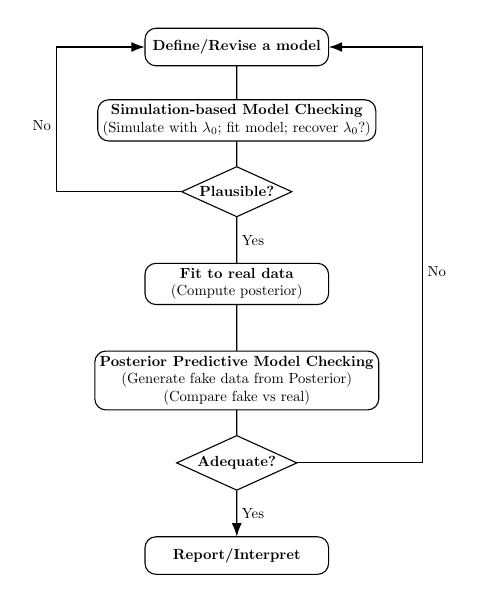
\begin{tikzpicture}[
 scale=0.53,
  every node/.style={transform shape}, 
  node distance=11mm,
  box/.style      ={rectangle, draw, rounded corners, align=center,
                    minimum width=44mm, minimum height=9mm},
  decision/.style ={diamond, aspect=2.2, draw, align=center, inner sep=1.4pt},
  ->, >=Latex
]

%--- Main process node ------------------------------------------------------
\node[box]      (model)   {\textbf{Define/Revise a model}};

\node[box]      (checking1)  [below=8mmof model] {\textbf{Simulation-based Model Checking} \\
(Simulate with $\lambda_0$; fit model; recover $\lambda_0$?)};

\node[decision] (pass1)   [below=6mm of checking1] {\textbf{Plausible?}};

\node[box]      (fit)     [below=of pass1]  {\textbf{Fit to real data}\\
(Compute posterior)};

\node[box]      (gen)     [below=of fit]    {\textbf{Posterior Predictive Model Checking}\\
(Generate fake data from Posterior)\\
(Compare fake vs real)};

\node[decision] (pass2)   [below=6mmof gen] {\textbf{Adequate?}};

\node[box]     (report)  [below=of pass2] {\textbf{Report/Interpret}};

%--- connection ------------------------------------------------------------
\draw (model)   -- (checking1)
      (checking1)  -- (pass1)
      (pass1)   -- node[right]{Yes}(fit)
      (fit)     -- (gen)
      (gen) -- (pass2)
      (pass2) -- node[right]{Yes}(report);

%--- Loopback ------------------------------------
\draw[->] (pass1.west) -- ++(-30mm,0) |- (model.west) node[pos=0.23, left]{No};
%\draw[->] (pass1.west) to[out=180,in=180,looseness=1.3] node[left]{No} (model.west);
\draw[->] (pass2.east) -- ++ (30mm,0 )|- (model.east) node[pos=0.23,right]{No};
\end{tikzpicture}}
\caption{General Bayesian workflow}
\label{flowchart}
\end{figure}

This workflow clearly distinguishes two levels of model checking.

First is the \textbf{Simulation-based Model Checking}, which evaluates structural identifiability based on known parameters~\cite{10.1093/bioinformatics/btp358}. Before fitting any real data, we can simulate pseudo-datasets using a fixed value $\lambda_0$, and then re-fit the model using the same procedure. If we successfully “recover” $\lambda_0$, this suggests that the model structure is sound; failure to do so implies structural flaws in the model, rendering downstream inferences on real data invalid~\cite{10.1093/bioinformatics/btp358, pub.1044073403}.

Second is the \textbf{Posterior Predictive Checking}, which evaluates the adequacy of the fitted model after conditioning on real data~\cite{https://doi.org/10.1002/ecm.1314}. In this approach, samples are drawn from the posterior distribution and used to generate replicated or “fake” datasets. These are then compared against the observed data to assess whether the model captures key statistical features. The underlying principle is that if data simulated from the posterior distribution differ systematically from the observed data, for example, in terms of censoring patterns or the distribution of event times, this indicates that the model fails to represent the true underlying process~\cite{62bfc978-09b1-3997-9776-380d0b45e9c2}. Bayesian methods naturally account for uncertainty by incorporating the full posterior distribution into this checking procedure~\cite{van2021bayesian}, ensuring that the evaluation reflects the range of plausible parameter values. Crucially, the discrepancies revealed by posterior predictive checks not only highlight structural inadequacies but also motivate targeted model extensions, guiding the development of more realistic survival models.


To implement this, we design a simulation procedure to generate synthetic survival datasets that preserve the censoring mechanism of the real data (see Algorithm 1)~\cite{ashhad2025generatingaccuratesyntheticsurvival}. The algorithm proceeds by drawing a posterior sample $\lambda^*$ and defining a suitable time window $[a, 0]$ to simulate individuals' entry times and latent event durations. For tractability, we assume that entry times are uniformly distributed across the observation window, corresponding to a constant entry rate during the study period. This allows us to generate a “virtual dataset” that matches the sample size and censoring structure of the original data, thereby enabling a rigorous comparison for posterior predictive model checking.
%%%%%%算法--------------
\begin{tcolorbox}[
  title  = {Algorithm 1: Simulating a Fake Survival Dataset (e.g., Posterior predictive model checking)},
  label={fake data},
   fonttitle  = \bfseries\footnotesize,
   fontupper=\footnotesize,
    %width = 0.9\textwidth,   
  box align = center, 
  colback = white,
  colframe=black,
   boxsep  = 3pt,
  left=4pt,
   right=4pt,
  top=5pt,
  bottom=4pt]
\textbf{Input}
\begin{itemize}[itemsep=1pt,parsep=0pt,topsep=2pt]
\item posterior samples $\{\lambda^{(s)}\}$ \hfill (obtained by fitting real data)
\item sample size $n$ \hfill (same size as the real data set)
\item start‑time range $[a,0]$ with $a<0$
\end{itemize}

\textbf{Algorithm}
\begin{enumerate}[itemsep=2pt,parsep=0pt,topsep=2pt]
  \item Choose a single $\lambda^\ast$ from posterior samples \hfill (e.g.\ posterior mean)
  \item For $i = 1,\dots,n$
          %\begin{minipage}[t]{\linewidth}
          \begin{enumerate}
            \item Draw latent duration: $y_i \sim \operatorname{Exp}(\lambda^\ast)$
            \item Draw start time: $T_i \sim \operatorname{Uniform}(a,0)$
            \item Compute leaving time: $t_i = T_i + y_i$
            \item Observed pair $(\text{time}_i,\text{event}_i)$ \[\begin{aligned}
\text{if } \quad t_i &< 0: &&&\text{(event occurred before now)}\\
  &&\quad  \text{event}_i=1, &&\text{(uncensored)}\\ 
  &&\quad \text{time}_i=y_i
   &\quad \\
&\text{else}: &&&\text{(event in the future)}\\
   &&\quad \text{event}_i=0, &&\text{(right censored)}\\ 
   &&\quad \text{time}_i=-T_i &&\text{(time already spent)}
   &\quad 
\end{aligned}\]
          \end{enumerate}
  \item Combine $(\text{time}_i,\text{event}_i)$ into a fake data set of size $n$.
\end{enumerate}
\end{tcolorbox}





\subsubsection{Model Checking via ECDF under Independent Censoring}
In model checking, to compare the overall distributional shapes of the real data and the simulated data, we use the empirical cumulative distribution function (ECDF) rather than histograms. Unlike histograms, ECDFs do not depend on subjective choices of bin widths and break points, thereby avoiding visual biases~\cite{berg2008data}. Moreover, an ECDF is a monotone right-continuous step function defined on $[0,\infty)$, which stably displays differences between samples over the entire time axis~\cite{arnold2011nonparametric, berg2008data}. Importantly, ECDFs can be plugged directly into distance statistics such as the Kolmogorov–Smirnov or Cramér–von Mises metrics~\cite{arnold2011nonparametric}, facilitating quantitative assessment of model fit.

In survival data, the observed duration is determined jointly by the latent event time $T\ge 0$ and the censoring time $C\ge 0$. The observed quantity is
$$
Y=\min(T,C),\qquad \delta=\mathbf 1\{T\le C\}.
$$
That is, we observe the event time only when it is uncensored; otherwise, we observe the censoring time. Consequently, we split the data into two subsamples, an “event subsample’’ with $\delta=1$ and a “censored subsample’’ with $\delta=0$, and compute ECDFs for each subsample separately.

Under independent (non-informative) censoring, i.e., $T\perp C$, the two subsamples may be viewed as arising from two conditional distributions~\cite{fleming2013counting}
\begin{itemize}
    \item for the event subsample ($\delta=1$), the observed values $Y=T$ follow the conditional distribution $T\mid(T\le C)$;
    \item for the censored subsample ($\delta=0$), the observed values $Y=C$ follow the conditional distribution $C\mid(C<T)$.
\end{itemize}
Let the event-subsample size be $n_1=\sum_i \delta_i$ and the censored-subsample size be $n_0=\sum_i (1-\delta_i)$. The corresponding empirical distribution functions are~\cite{fleming2013counting, arnold2011nonparametric}
\begin{equation}
    \widehat H_{\text{event}}(t)
=\frac{1}{n_1}\sum_{i:\,\delta_i=1}\mathbf 1\{Y_i\le t\},\qquad
\widehat H_{\text{cens}}(t)
=\frac{1}{n_0}\sum_{i:\,\delta_i=0}\mathbf 1\{Y_i\le t\},\qquad t\ge 0.
\end{equation}
By the Glivenko–Cantelli theorem~\cite{tucker1959generalization}, as sample sizes grow, these ECDFs converge uniformly to their respective target distribution functions
\begin{align}
\widehat H_{\text{event}}(t) &\xrightarrow{\text{uniformly in } t} H_{\text{event}}(t) := \Pr(T \le t \mid T \le C) \\
\widehat H_{\text{cens}}(t) &\xrightarrow{\text{uniformly in } t} H_{\text{cens}}(t) := \Pr(C \le t \mid C < T)
\end{align}
In summary, by splitting the data into event and censored subsamples and plotting their empirical distribution functions $\widehat H_{\text{event}}$ and $\widehat H_{\text{cens}}$, we can evaluate model fit within a unified framework along both dimensions.

%\subsection{Posterior predictive CDF}
%\input{MSc_Statistics_Research_Report_paper/section/Methods_subsection/posterior predictive cdf }


























\section{Results}
\label{sec:results}
\subsection{Posterior Inference under the Extended Model}



\subsection{Marginalization and Consistency Check}




\subsection{Baseline Exponential Model Fit}
\label{ecdf的分析}




\subsection{Posterior Predictive Model Checking}

\section{Discussion}
\label{sec:discussion}
The preceding results examined various aspects of model fit, and Sections~\ref{res:post_contour} and~\ref{res:marginal} highlight an especially intriguing finding. Specifically, the marginal posterior of $\lambda$ is unaffected by the prior choice on $A$, as long as the support condition $A \geq y_{\max}$ is satisfied. This separability is unusual in multi-parameter Bayesian survival models, where parameters typically remain entangled and sensitive to prior assumptions. Here, however, the inference for the event-rate parameter $\lambda$ remains robust, while $A$ serves only to capture the structural features of the censoring mechanism. In practical terms, this means $\lambda$ can always be stably estimated, while $A$ captures censoring structure without distorting inference on the underlying hazard rate. 

While this theoretical robustness is reassuring, posterior predictive checks simultaneously reveal practical shortcomings of the exponential baseline. As shown in Section~\ref{res: model checking}, the constant hazard assumption fails to capture the empirical feature of the data, namely a “steep early rise followed by a gradual decline.” This results in a systematic underestimation of event occurrences in the mid-range. To address this mismatch, it is natural to consider alternative distributions, especially those that allow hazards to vary over time and possibly take non-monotonic forms.

Before moving to such flexible specifications, however, it is natural to first reflect on a monotone alternative: the Weibull model. Although Weibull introduces time dependence, its single shape parameter limits flexibility, making it difficult to accommodate both the sharp early risk and the smoother decline in later periods (as illustrated more clearly in the supplementary figures, such an adjustment does not lead to noticeable improvement). Hence, models with monotone hazards are not suitable for this dataset. This reflection points toward a more promising direction: models that allow non-monotone and locally curved baseline hazards.

A natural candidate is the piecewise-constant hazard (PWE) model. Dividing time into intervals permits the hazard to vary flexibly across segments, thereby directly capturing the “early steep, later flat” turnover pattern observed in the data. Here, I illustrate this approach with a simplified version using six segments, while keeping the observation window fixed at $A=179$ for comparability with the exponential model. The posterior predictive results show that the ECDF of event times improves markedly, indicating that such models align more closely with the structure of the data.
\begin{figure}[H]
    \centering
    \includegraphics[height=6cm, width=0.75\textwidth]{images/piece6_ecdf_comparison.pdf}
    \caption{{\small Posterior predictive ECDFs of event times (left) and censored durations (right) under a six-segment piecewise-constant hazard model (cuts at 40, 75, 105, 120, 160, 200), with $A=179$ fixed for comparability.}}
    \label{fig:ppc_map}
\end{figure}
However, this exercise also reveals another issue that even under the PWE framework, the fit for censoring remains problematic. The observed censoring ECDF lies systematically above the simulated one. This discrepancy does not arise from the event process but rather from the censoring mechanism. In the current PPC setting, we assume uniform entry over $[0, A]$, such that censoring is entirely administrative. In reality, however, recruitment may not be uniform—for instance, if the company recruits heavily in later periods, this would generate more early censoring. This explains the “excess censoring” observed in the real data and suggests that future work should incorporate entry mechanisms informed by the company’s operational context.

Finally, it is important to note that modeling choices depend on research objectives. If the aim is to characterize overall turnover trends, improving the baseline hazard and censoring mechanism may already provide useful conclusions. But if the goal is to predict turnover risk at the individual level, covariates must be incorporated to account for heterogeneity across employees.




\section*{Endmatter} \label{sec:endmatter}
The employee turnover dataset described in Section~\ref{sec: data} is publicly available at \href{https://www.kaggle.com/datasets/davinwijaya/employee-turnover/data}{Kaggle}, and all analysis code for reproducing the results is provided at \href{https://github.com/zooogi/Statistics-Research-Project.git}{GitHub}.

%=========================================================
%
%
%
% Students should not edit below here 
%
%
%
%=========================================================

%=========================================================
%% Create bibliography
%
% - Add your references by modifying the file `refs.bib`
%
%=========================================================

\clearpage

%%References part of the main text
% References: modify the file refs.bib
\bibliographystyle{unsrtnat} 
\bibliography{refs}


\clearpage

%=========================================================
%% Create supplementary material 
%
%
% - Providing supplementary materials to your report is voluntary and will not normally be read by your examiners.
% - If you wish to include supplementary materials, add these by modifying the file 
%   `supplementary.tex`
% - otherwise deactive the include command below
%
%
%=========================================================

%% reset page counter and start appendix pages numbering
\pagenumbering{arabic}
\renewcommand*{\thepage}{Supplementary Material Page \arabic{page}}
\renewcommand{\thesection}{\Alph{section}}
%% Supplementary Material goes here
\appendix
\pagebreak
\section*{Supplementary Materials}

\setcounter{figure}{0}
\setcounter{table}{0}

\renewcommand{\thefigure}{S\arabic{figure}}
\renewcommand{\thetable}{S\arabic{table}}

\begin{figure}[H]
  \centering
  \includegraphics[width=0.8\textwidth]{images/simulation-based_model_check.png}
  \caption{{\small Posterior distribution of $\lambda$ from the simulation-based model check with $\lambda=0.05$.}}
  \label{fig:posterior_s1}
\end{figure}
%=========================================================


\end{document}
